\chapter{Antecedentes y estado del arte}
\label{chap:antecedentes}

\drop{S}{aber} que los datos condicionan la calidad de un modelo de \ac{IA} no
basta si no se dispone de una forma sistemática de medirlo.  Durante las
últimas décadas, la investigación ha producido dos tipos de respuesta: marcos
conceptuales y estándares internacionales que definen qué es la calidad de
datos, y herramientas que permiten medirla de forma automatizada.  Este capítulo
revisa ambos frentes para situar \dataqual en su contexto: qué se sabe sobre
la calidad de datos en \ac{IA}, qué normas la regulan, qué herramientas ya
existen y por qué ninguna cubre exactamente el espacio que \dataqual ocupa.

Para ello, el capítulo se organiza en tres bloques.  La
sección~\ref{sec:importancia-calidad} revisa la importancia de la calidad de
datos en proyectos de \ac{IA} y sus marcos conceptuales fundacionales.  La
sección~\ref{sec:marco-normativo} examina el marco normativo de estándares
\ac{ISO} aplicables, incluida la taxonomía de \ac{ISO}/\ac{IEC}~5259-2
(sección~\ref{sec:alcance-metodologico}) que delimita el alcance del proyecto.
Por último, la sección~\ref{sec:estado-arte} analiza las soluciones
existentes y las compara sistemáticamente
(sección~\ref{sec:analisis-comparativo}), de lo que se desprende el hueco que
\dataqual viene a cubrir, y reseña otras herramientas del ecosistema.


%% =========================================================================
\section[Importancia de la calidad de datos en IA]{La importancia de la calidad de datos en proyectos de~\ac{IA}}
\label{sec:importancia-calidad}
%% =========================================================================

La calidad de los datos cuenta con una base teórica consolidada que conviene
revisar antes de abordar su medición.  Esta sección recorre los marcos
conceptuales fundacionales que la definieron, su impacto económico y de
proceso, y el cambio de enfoque que supone el paradigma
\emph{data-centric AI}.

\subsection{Marcos conceptuales fundacionales}

Los trabajos seminales de Wang y Strong~(\citeyear{wang1996}) establecieron un marco
conceptual para la calidad de datos basado en cuatro categorías
fundamentales, sintetizadas en la figura~\ref{fig:wang-strong}: la
\emph{calidad intrínseca}, que recoge las propiedades del dato en sí
mismo (precisión, objetividad, credibilidad y reputación); la \emph{calidad
contextual}, que mide su adecuación a la tarea en la que se utiliza
(relevancia, valor añadido, completitud, cantidad apropiada y oportunidad
temporal); la \emph{calidad representacional}, asociada a la forma en que
el dato se presenta al usuario (interpretabilidad, facilidad de
comprensión, concisión y consistencia); y la \emph{accesibilidad}, que
cubre la disponibilidad del dato y la seguridad en su acceso.

\begin{figure}[H]
  \centering
  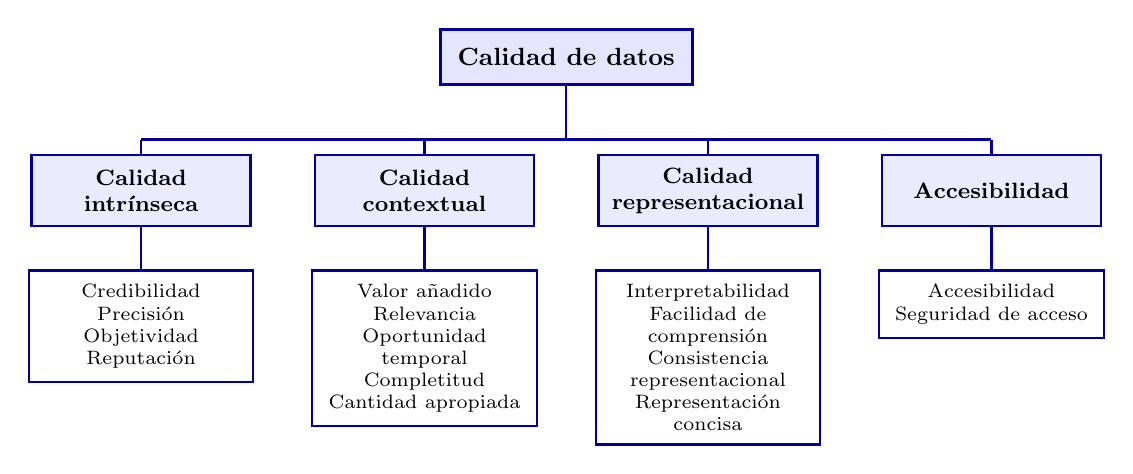
\begin{tikzpicture}[
    root/.style={
      rectangle, draw=blue!60!black, very thick, fill=blue!10,
      minimum width=3.2cm, minimum height=0.7cm,
      align=center, font=\small\bfseries
    },
    cat/.style={
      rectangle, draw=blue!60!black, thick, fill=blue!8,
      text width=2.5cm, minimum height=0.9cm,
      align=center, font=\footnotesize\bfseries,
      inner sep=4pt
    },
    attrs/.style={
      rectangle, draw=blue!60!black, thick, fill=white,
      text width=2.5cm, align=center,
      font=\scriptsize, inner sep=5pt
    },
    link/.style={-, thick, blue!60!black}
  ]
    \node[root] (root) at (0,0) {Calidad de datos};

    \node[cat] (intrin) at (-5.4,-1.7) {Calidad\\intrínseca};
    \node[cat] (cont)   at (-1.8,-1.7) {Calidad\\contextual};
    \node[cat] (repr)   at ( 1.8,-1.7) {Calidad\\representacional};
    \node[cat] (acc)    at ( 5.4,-1.7) {Accesibilidad};

    \node[attrs, anchor=north] (a-intrin) at (-5.4,-2.7) {%
      Credibilidad\\Precisión\\Objetividad\\Reputación};
    \node[attrs, anchor=north] (a-cont)   at (-1.8,-2.7) {%
      Valor añadido\\Relevancia\\Oportunidad temporal\\Completitud\\Cantidad apropiada};
    \node[attrs, anchor=north] (a-repr)   at ( 1.8,-2.7) {%
      Interpretabilidad\\Facilidad de comprensión\\Consistencia representacional\\Representación concisa};
    \node[attrs, anchor=north] (a-acc)    at ( 5.4,-2.7) {%
      Accesibilidad\\Seguridad de acceso};

    \draw[link] (root.south) -- (0,-1.05);
    \draw[link] (-5.4,-1.05) -- (5.4,-1.05);
    \draw[link] (intrin.north) -- (-5.4,-1.05);
    \draw[link] (cont.north)   -- (-1.8,-1.05);
    \draw[link] (repr.north)   -- ( 1.8,-1.05);
    \draw[link] (acc.north)    -- ( 5.4,-1.05);

    \draw[link] (intrin.south) -- (a-intrin.north);
    \draw[link] (cont.south)   -- (a-cont.north);
    \draw[link] (repr.south)   -- (a-repr.north);
    \draw[link] (acc.south)    -- (a-acc.north);
  \end{tikzpicture}
  \caption[Marco conceptual de calidad de datos de Wang y Strong]{Marco
    conceptual de calidad de datos: cuatro categorías y sus atributos
    asociados. Adaptado de Wang y Strong~(\citeyear{wang1996}).}
  \label{fig:wang-strong}
\end{figure}

El estándar \ac{ISO}/\ac{IEC}~25012 recoge el vocabulario conceptual de este
marco (completitud, exactitud, consistencia y accesibilidad) rearticulándolo
en un modelo orientado a sistemas de información que distingue entre
características inherentes al dato y características dependientes del entorno
tecnológico que lo aloja.

\subsection{Impacto económico y de proceso}

Redman~(\citeyear{redman1998}) estimó que los errores en datos consumen
entre el 8\,\% y el 12\,\% de los ingresos de una organización, pudiendo
alcanzar entre el 40\,\% y el 60\,\% de los gastos operativos en empresas
de servicios; investigaciones posteriores del mismo
autor~(\citeyear{redman2001}) elevaron ese rango hasta el 25\,\% en
sectores con mayor dependencia de datos.  Estudios posteriores del MIT
Information Quality Program y del \ac{DMBOK}~\citep{dmbok2017} han
reproducido estas cifras con resultados similares.  Trabajos recientes
confirman que el problema sigue plenamente vigente: la revisión de
Ehrlinger y Wöß~(\citeyear{ehrlinger2022}) documenta la proliferación de
herramientas de medición y monitorización de calidad de datos como
respuesta a este coste sostenido.

A esta dimensión económica se suma una dimensión de proceso.  Según
CrowdFlower~\citep{crowdflower2016}, los científicos de datos dedicaban
en 2016 cerca del 80\,\% de su tiempo a preparación y limpieza de datos;
encuestas más recientes~\citep{anaconda2022} sitúan esa cifra en torno
al 38\,\%, pero sigue siendo la tarea que más tiempo consume, por encima
de visualización (13\,\%) y entrenamiento de modelos (9\,\%).  El
fenómeno se reconoce como un problema estructural, ya que las \emph{Data
Cascades} descritas por Sambasivan et al.~(\citeyear{sambasivan2021}) y
sus consecuencias prácticas se desarrollan en la
sección~\ref{sec:motivacion}, lo que refuerza la necesidad de
herramientas automatizadas de diagnóstico de calidad.

\subsection{El paradigma data-centric AI}

Ng~(\citeyear{ng2021datacentric}) acuñó el término \emph{data-centric AI}
para describir un giro metodológico respecto al enfoque tradicional
\emph{model-centric}: en lugar de mantener los datos fijos y mejorar el
algoritmo, se mantiene el modelo fijo y se mejora sistemáticamente el dataset.
La premisa es contundente: en la mayoría de proyectos reales de \ac{IA},
invertir esfuerzo en los datos produce ganancias de rendimiento mayores que
afinar la arquitectura del modelo.

Diversas iniciativas han consolidado este paradigma en la comunidad:

\begin{itemize}
  \item La \emph{Data-Centric AI Competition}, organizada por Andrew Ng y
    Landing AI, en la que los participantes compiten mejorando un dataset fijo
    en lugar de un modelo fijo.
  \item \emph{DataPerf}, una iniciativa de MLCommons que proporciona
    \emph{benchmarks} centrados en la calidad de datos para sistemas de
    \ac{ML}.
  \item El área de investigación \emph{Data Quality for AI}, que explora
    métricas de calidad específicas para conjuntos de datos destinados al
    entrenamiento de modelos.
\end{itemize}

El paradigma data-centric subraya además que los propios datos son
fuente recurrente de sesgo sistemático: los casos documentados
(reconocimiento facial, contratación, reincidencia, valoración
inmobiliaria) se discuten en la sección~\ref{sec:motivacion} y conectan
con las dimensiones de equilibrio de clases, representatividad y
actualidad recogidas por \ac{ISO}/\ac{IEC}~5259.


%% =========================================================================
\section{Marco normativo: estándares \ac{ISO}/\ac{IEC}}
\label{sec:marco-normativo}
%% =========================================================================

La evaluación de la calidad de datos se enmarca dentro de un conjunto de
estándares internacionales publicados por \ac{ISO}/\ac{IEC}. \dataqual toma como
referencia conceptual los estándares \ac{ISO}/\ac{IEC}~25012 e
\ac{ISO}/\ac{IEC}~25024, que definen respectivamente el modelo de calidad de datos
y sus métricas de medición, y se alinea de forma explícita con
\ac{ISO}/\ac{IEC}~5259, el estándar específico para calidad de datos en analítica
e \ac{IA}, cuya taxonomía de características estructura las decisiones de
alcance del proyecto.  La Figura~\ref{fig:estandares-contexto} sitúa
\dataqual respecto a estos estándares y al marco normativo europeo, indicando
el papel que cada uno desempeña en la plataforma; las subsecciones siguientes
desarrollan cada referencia.

\begin{figure}[htbp]
  \centering
  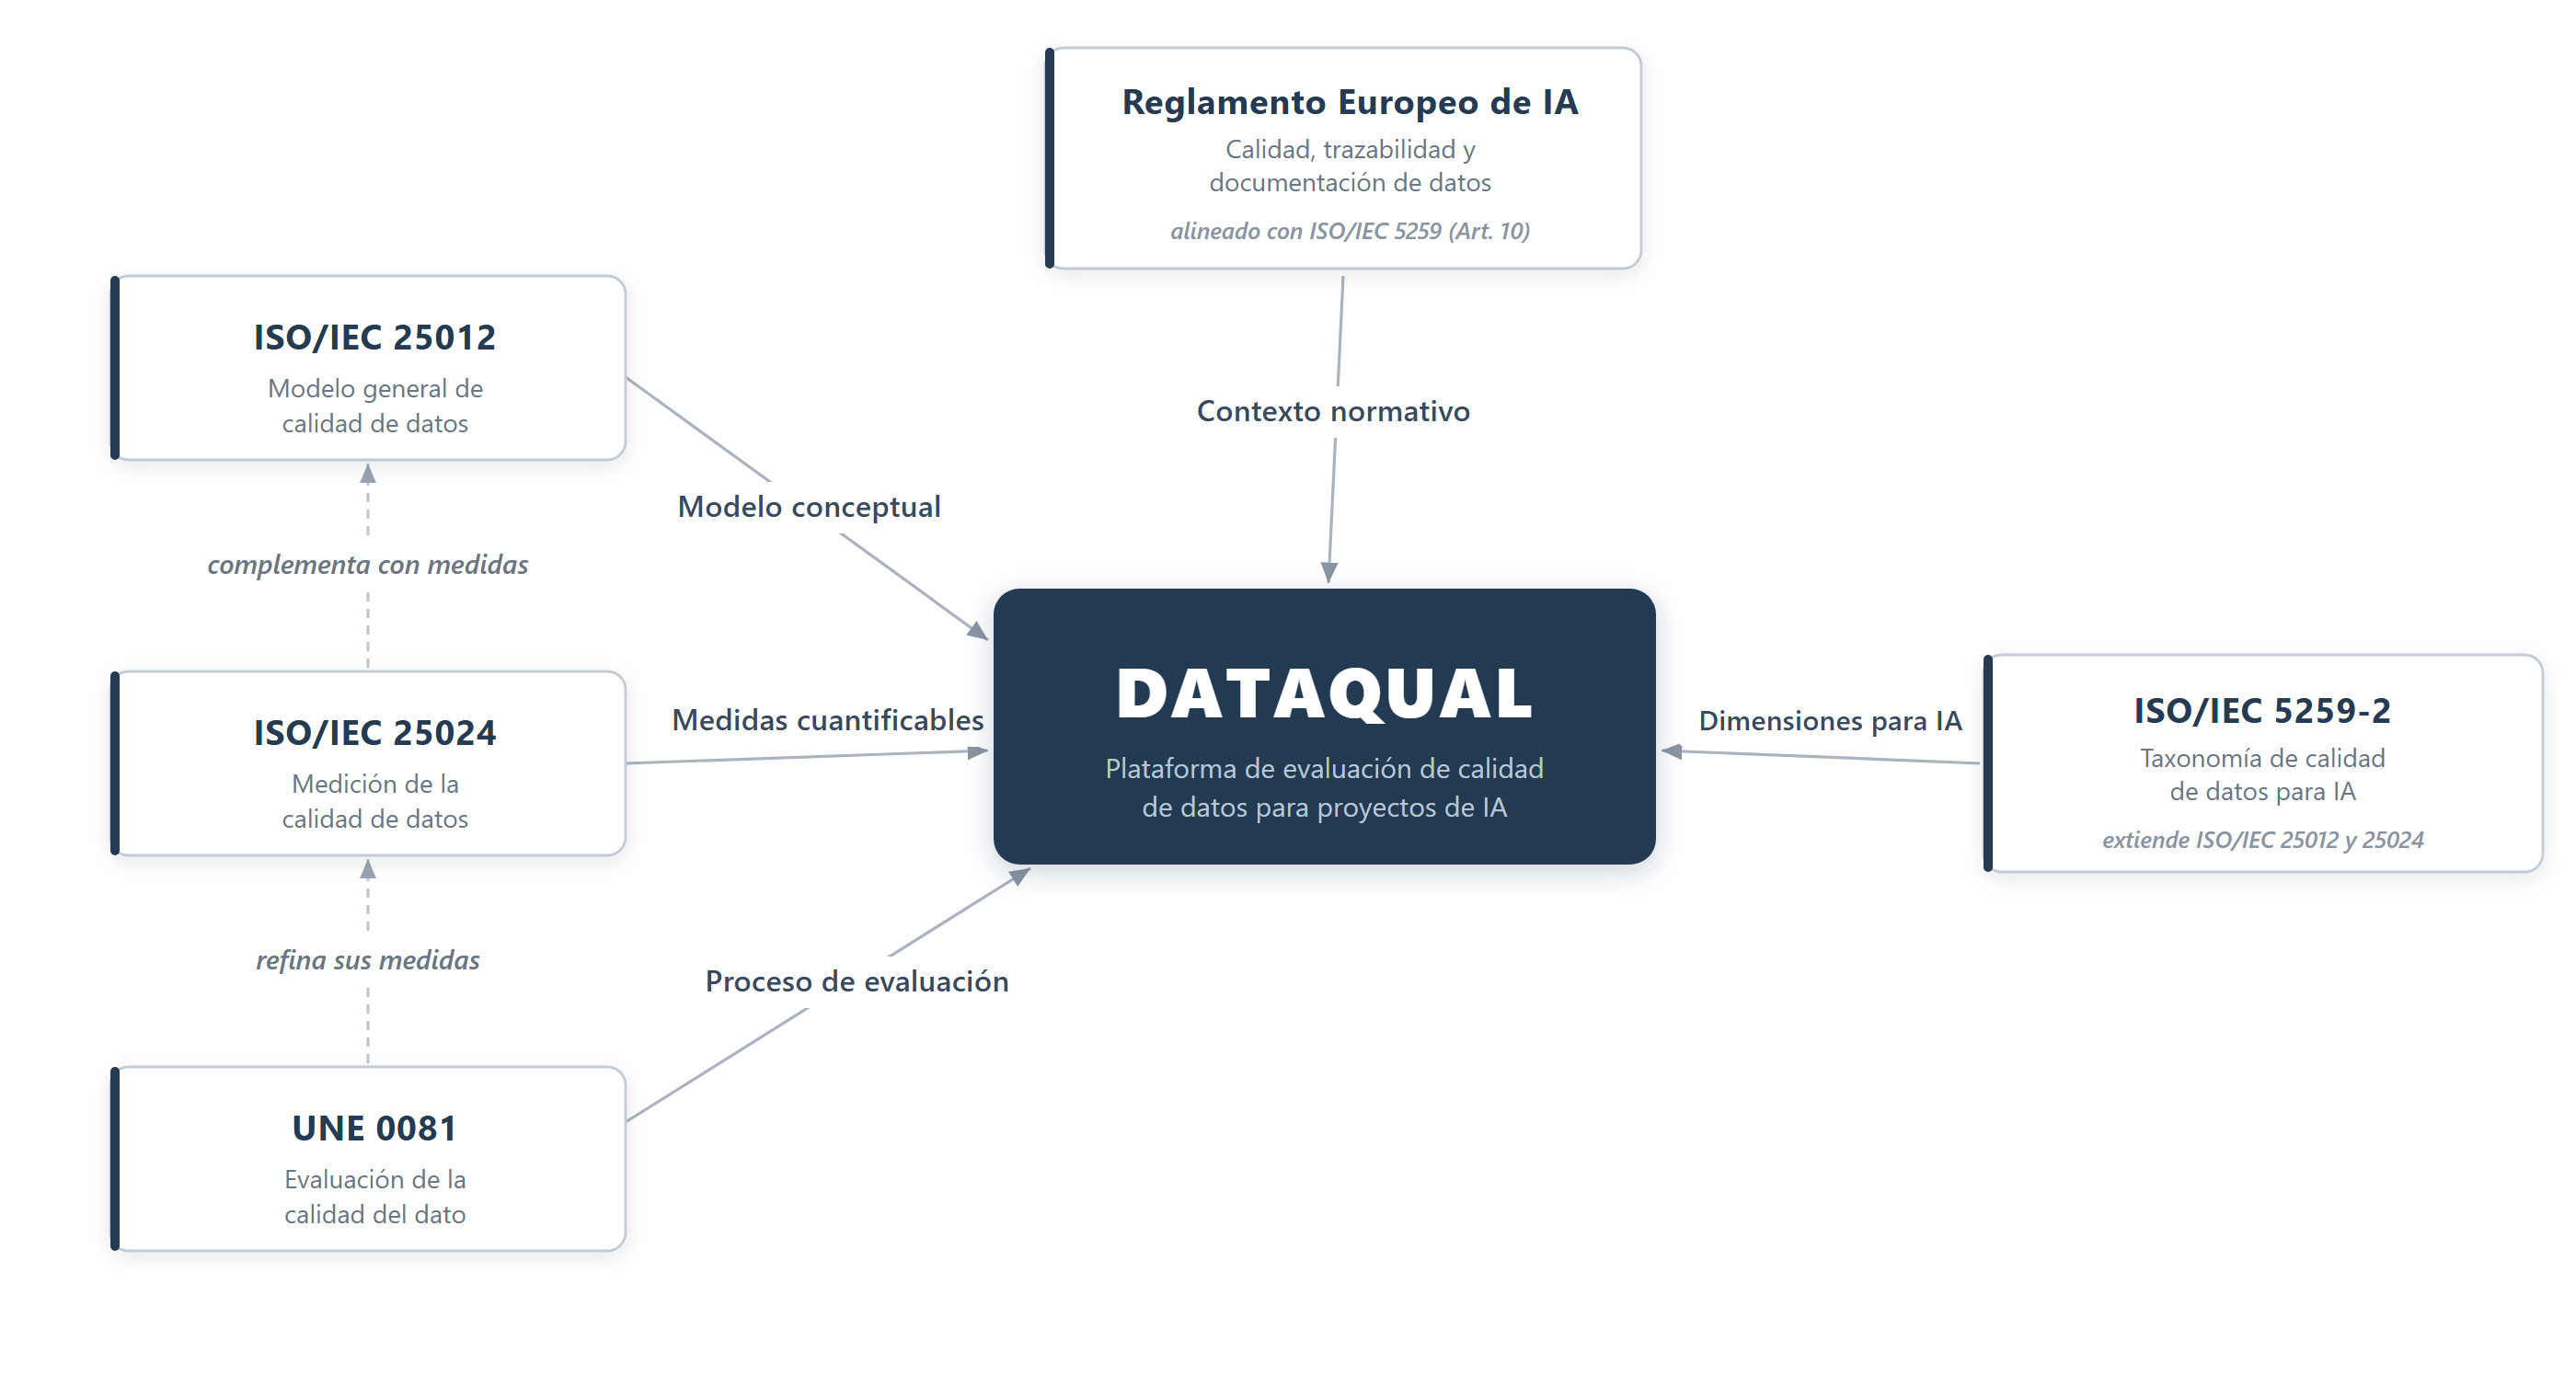
\includegraphics[width=\textwidth]{figures/img/estandares-contexto.png}
  \caption[Contexto normativo de \dataqual]{Relación de \dataqual con los
    estándares de calidad de datos (\ac{ISO}/\ac{IEC}~25012, 25024 y 5259-2;
    \ac{UNE}~0081) y con el marco normativo europeo, junto con el papel que
    cada referencia desempeña en la plataforma.}
  \label{fig:estandares-contexto}
\end{figure}

\subsection{\ac{ISO}/\ac{IEC} 25012: Modelo de calidad de datos}
\label{sec:iso25012}

El estándar \ac{ISO}/\ac{IEC} 25012~\citep{iso25012} forma parte de la familia
\ac{SQuaRE} y define un modelo de calidad de datos que comprende 15
características distribuidas en tres agrupaciones. La \textbf{calidad
inherente} recoge cinco propiedades intrínsecas del dato (exactitud,
completitud, consistencia, credibilidad y actualidad, \emph{currentness})
evaluables con independencia del sistema que los almacena. La
\textbf{calidad dependiente del sistema} comprende tres propiedades
(disponibilidad, portabilidad y recuperabilidad) determinadas por el contexto
tecnológico. Una tercera agrupación engloba siete características a la vez
inherentes y dependientes del sistema (accesibilidad, conformidad,
confidencialidad, eficiencia, precisión, trazabilidad y comprensibilidad),
cuya evaluación requiere tanto el análisis del dato como el conocimiento del
entorno que lo gestiona.

\dataqual implementa métricas que cubren las principales características
inherentes del estándar, añadiendo además métricas específicas para proyectos
de \ac{IA} que no están contempladas en la norma. Conviene precisar que
\ac{ISO}/\ac{IEC}~25012 define las \emph{características} de calidad, mientras
que \ac{ISO}/\ac{IEC}~25024 las descompone en \emph{medidas} concretas y
cuantificables; cada métrica de \dataqual se ancla, por tanto, a una medida
específica de 25024 y no a la característica genérica. El
Cuadro~\ref{tab:iso25012-dataqual} muestra esa correspondencia, indicando
entre paréntesis la medida de 25024 sobre la que se pone el foco.

\begin{table}[htbp]
  \centering
  \caption{Correspondencia entre las características de calidad de \ac{ISO}/\ac{IEC}~25012 e \ac{ISO}/\ac{IEC}~5259-2, sus medidas en \ac{ISO}/\ac{IEC}~25024 y las métricas implementadas en \dataqual}
  \label{tab:iso25012-dataqual}
  \footnotesize
  \newcommand{\tblnote}{\textsuperscript{a}}%
  \begin{tabularx}{\textwidth}{l l l >{\raggedright\arraybackslash}X}
    \toprule
    \textbf{Característica} & \textbf{Norma} & \textbf{Métrica \dataqual} & \textbf{Implementación} \\
    \midrule
    \multicolumn{4}{l}{\emph{Modelo general de calidad de datos (\ac{ISO}/\ac{IEC}~25012; medidas en 25024)}} \\
    \midrule
    Completitud          & \ac{ISO}~25012; 25024 (Compl\_04)  & \texttt{completeness}          & Ratio de valores no nulos por columna \\[10pt]
    Exactitud            & \ac{ISO}~25012; 25024 (Exac\_01)   & \texttt{syntactic\_accuracy}    & Conformidad con patrones de formato \\[10pt]
    Consistencia\tblnote & \ac{ISO}~25012; 5259-2             & \texttt{logical\_consistency}   & Reglas IF-THEN entre columnas \\[10pt]
    Consistencia\tblnote & \ac{ISO}~25012; 25024 (Cons\_03)   & \texttt{uniqueness}             & Detección de registros duplicados \\[10pt]
    Actualidad           & \ac{ISO}~25012           & \texttt{currentness}            & Antigüedad del dato más reciente \\
    \midrule
    \multicolumn{4}{l}{\emph{Características propias de los conjuntos de datos para \ac{IA} (\ac{ISO}/\ac{IEC}~5259-2)}} \\
    \midrule
    Equilibrio (Balance) & \ac{ISO}~5259-2          & \texttt{class\_balance}         & Entropía de Shannon \\[10pt]
    Diversidad           & \ac{ISO}~5259-2          & \texttt{diversity}              & Cobertura de valores esperados por columna \\
    \bottomrule
  \end{tabularx}
  \medskip\par\footnotesize\raggedright
  \textsuperscript{a}~La consistencia se operacionaliza en dos métricas: coherencia lógica
  entre columnas y ausencia de duplicados, siguiendo las sub-dimensiones
  Con-ML-4 y Con-ML-1 de \ac{ISO}/\ac{IEC}~5259-2 respectivamente.
  \par\smallskip
  Los códigos entre paréntesis identifican la medida concreta de
  \ac{ISO}/\ac{IEC}~25024: Compl\_04 (completitud de valores de datos),
  Exac\_01 (exactitud sintáctica de los datos) y Cons\_03 (riesgo de
  inconsistencia por duplicación del valor de los datos).
\end{table}

\subsection{\ac{ISO}/\ac{IEC} 5259: Calidad de datos para analítica e IA}
\label{sec:iso5259}

El estándar \ac{ISO}/\ac{IEC} 5259~\citep{iso5259} aborda específicamente la
calidad de datos en contextos de analítica e inteligencia artificial y
aprendizaje automático. Su Parte~2 no parte de cero: se construye sobre
\ac{ISO}/\ac{IEC}~25012~\citep{iso25012} e \ac{ISO}/\ac{IEC}~25024~\citep{iso25024},
de las que importa el modelo de calidad y sus medidas, y las extiende con
características propias de los conjuntos de datos para \ac{IA} (como la
diversidad o la representatividad). La serie consta de cinco partes, de las
cuales la Parte~2 (medidas de calidad de datos) fue publicada en noviembre de
2024~\citep{iso5259}: \textbf{Parte~1. Visión general}, que establece los
conceptos fundamentales y el vocabulario común; \textbf{Parte~2. Métricas de
calidad de datos}, que define métricas cuantitativas estandarizadas para
evaluar la calidad de datos destinados a sistemas de \ac{IA}; \textbf{Parte~3.
Gestión de datos}, que cubre la gestión de conjuntos de datos, incluyendo
versionado y trazabilidad; \textbf{Parte~4. Marco de procesos}, que describe el
flujo de evaluación integrado en el ciclo de vida de un proyecto de \ac{IA}; y
\textbf{Parte~5. Verificación y validación}, que establece los requisitos para
verificar y validar los procesos y resultados de evaluación de calidad de datos.

\dataqual se alinea con este estándar en varios aspectos: proporciona métricas
cuantitativas estandarizadas (Parte~2), implementa gestión de datasets con
versionado (Parte~3) y ofrece un flujo de evaluación integrado en el ciclo de
vida del proyecto (Parte~4).

Desde el punto de vista del alcance, la contribución más relevante de
\ac{ISO}/\ac{IEC} 5259-2 es su taxonomía de características de calidad, que se
detalla a continuación y constituye el marco conceptual sobre el que se delimita
el alcance técnico de \dataqual.

\subsection[Taxonomía de \ac{ISO}/\ac{IEC} 5259-2]{Taxonomía de \ac{ISO}/\ac{IEC} 5259-2}
\label{sec:alcance-metodologico}

\ac{ISO}/\ac{IEC}~5259-2~\citep{iso5259} organiza las características de calidad
de datos para analítica e \ac{IA} en cuatro grupos según su naturaleza y su
grado de dependencia del contexto tecnológico.  Esta taxonomía constituye
la base conceptual sobre la que, en el capítulo de resultados
(sección~\ref{sec:instanciacion-iso5259}), se discutirán las decisiones de
cobertura y priorización adoptadas en \dataqual.  La
Figura~\ref{fig:iso5259-taxonomia} sintetiza visualmente las cuatro
agrupaciones y sus dimensiones; los párrafos que siguen elaboran cada una
de ellas.

\begin{figure}[htbp]
  \centering
  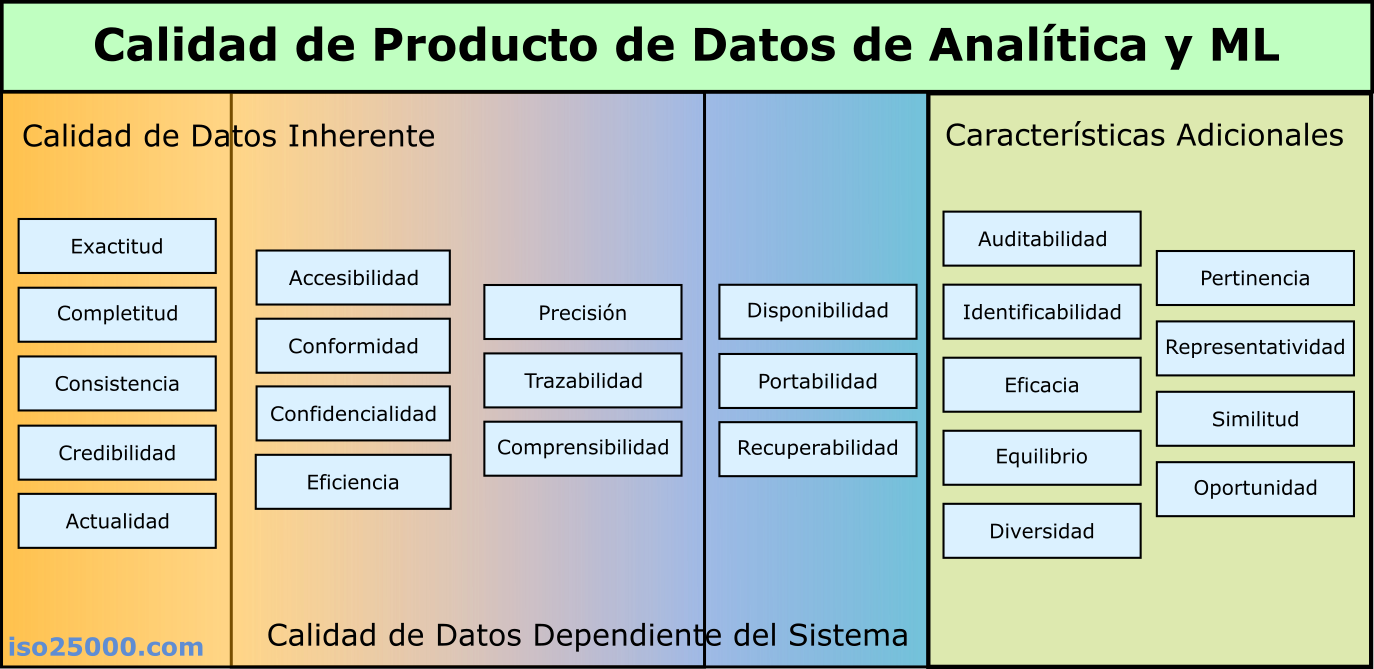
\includegraphics[width=0.95\textwidth]{figures/img/iso5259-taxonomia.png}
  \caption[Taxonomía de características de calidad de \ac{ISO}/\ac{IEC}~5259-2]{%
    Taxonomía de características de calidad de datos para analítica e
    \ac{IA} según \ac{ISO}/\ac{IEC}~5259-2. Fuente: \cite{iso25000web}.}
  \label{fig:iso5259-taxonomia}
\end{figure}

\begin{itemize}
  \item \textbf{Características inherentes} (5): exactitud
    (\emph{accuracy}), completitud (\emph{completeness}), consistencia
    (\emph{consistency}), credibilidad (\emph{credibility}) y actualidad
    (\emph{currentness}). Son propiedades intrínsecas del dato, evaluables
    a partir del análisis de sus valores sin necesidad de conocer el sistema
    que lo aloja.

  \item \textbf{Características mixtas} (7): accesibilidad
    (\emph{accessibility}), conformidad (\emph{compliance}), eficiencia
    (\emph{efficiency}), precisión (\emph{precision}), trazabilidad
    (\emph{traceability}), confidencialidad (\emph{confidentiality}) y
    comprensibilidad (\emph{understandability}). Dependen tanto de las
    propiedades del dato como del contexto del sistema que lo gestiona.

  \item \textbf{Características dependientes del sistema} (3):
    disponibilidad (\emph{availability}), portabilidad (\emph{portability})
    y recuperabilidad (\emph{recoverability}). Vienen determinadas
    exclusivamente por la infraestructura tecnológica de la organización.

  \item \textbf{Características adicionales para IA/ML} (9): equilibrio
    (\emph{balance}), diversidad (\emph{diversity}), efectividad
    (\emph{effectiveness}), identificabilidad (\emph{identifiability}),
    relevancia (\emph{relevance}), representatividad
    (\emph{representativeness}), similitud (\emph{similarity}), puntualidad
    (\emph{timeliness}) y auditabilidad (\emph{auditability}). Abordan
    necesidades específicas del aprendizaje automático que los marcos
    generalistas de calidad de datos no contemplan.
\end{itemize}


\subsection[\ac{UNE} 0081: evaluación de la calidad del dato]{\ac{UNE} 0081: evaluación de la calidad del dato}
\label{sec:une0081}

En el contexto español, la norma \ac{UNE} 0081~\citep{une0081}, publicada
en 2023 por la Asociación Española de Normalización dentro de la familia
\ac{UNE} 0078--0081 sobre gobierno, gestión y calidad del dato (Comité Técnico
de Normalización CTN~320/SC~1), complementa este ecosistema orientándose
a mejorar la aplicabilidad de la familia \ac{SQuaRE}: propone un modelo de
evaluación de la calidad del dato que toma las características de
\ac{ISO}/\ac{IEC}~25012 y las medidas de \ac{ISO}/\ac{IEC}~25024, que precisa
con criterios de cálculo más concretos, formalizando así un procedimiento
operativo para su aplicación en organizaciones.  \dataqual se alinea con su enfoque al adoptar
las medidas cuantitativas de \ac{ISO}/\ac{IEC}~25024 dentro de un proceso
reproducible de evaluación con trazabilidad y comparación entre
ejecuciones, lo que facilita la auditoría de resultados en entornos
sujetos a esta normativa.

\subsection{\ac{ISO}/\ac{IEC} 25024: Medición de la calidad de datos}
\label{sec:iso25024}

El estándar \ac{ISO}/\ac{IEC} 25024~\citep{iso25024} complementa al 25012
proporcionando métricas concretas y fórmulas de medición para cada
característica de calidad. De este modo, se pasa de un modelo conceptual
abstracto a un conjunto de indicadores cuantificables.

\dataqual pone el foco en tres medidas concretas de este estándar: la
\textbf{completitud de valores de datos} (Compl\_04: proporción de valores no
nulos sobre el total de valores esperados en una columna o dataset), la
\textbf{exactitud sintáctica de los datos} (Exac\_01: proporción de valores
que se ajustan a un patrón o formato predefinido mediante expresiones
regulares, rangos numéricos o conjuntos de valores permitidos) y el
\textbf{riesgo de inconsistencia por duplicación} (Cons\_03), que se
operacionaliza como detección de registros duplicados. La elección de estas
tres medidas, frente al amplio catálogo que 25024 define para cada
característica, responde al criterio de priorizar las de mayor impacto y
aplicabilidad directa sobre datasets tabulares.

La adopción de estas fórmulas estandarizadas garantiza que los resultados de
\dataqual sean comparables con los obtenidos por otras herramientas que
implementen el mismo estándar, facilitando la comparabilidad entre
herramientas y la auditoría de resultados.

El Reglamento Europeo de Inteligencia Artificial~\citep{aiact2024} refuerza
la relevancia del conjunto de estándares descrito en esta sección: exige que
las organizaciones puedan demostrar la calidad y trazabilidad de los datos
utilizados en sus modelos, lo que convierte la evaluación estandarizada de
calidad de datos en una necesidad no solo técnica, sino también de
cumplimiento normativo. De hecho, su artículo~10 sobre gobernanza de datos
sitúa a la serie \ac{ISO}/\ac{IEC}~5259 como referencia para evaluar dicha
calidad, hasta el punto de estar prevista como norma armonizada para acreditar
su cumplimiento.


%% =========================================================================
\section{Soluciones similares existentes}
\label{sec:estado-arte}
%% =========================================================================

Para contextualizar la contribución de \dataqual es necesario conocer qué
existe ya. Las herramientas descritas a continuación representan las
soluciones de referencia en evaluación de calidad de datos; sus fortalezas
y sus límites definen el espacio en el que \dataqual opera.

\begin{itemize}
  \item \textbf{Great Expectations}~\citep{greatexpectations} es una biblioteca
    de código abierto en Python para definir y validar «expectativas»
    (\emph{expectations}): aserciones declarativas sobre las propiedades que se
    esperan de los datos, como «esta columna no debe contener valores nulos».
    Cuenta con un ecosistema maduro y comunidad activa, soporta múltiples
    \emph{backends} de ejecución (Pandas, Spark, \ac{SQL}) y genera
    documentación visual automática de los resultados (\emph{Data Docs}). Como
    contrapartida, es \emph{code-first} y exige conocimientos de Python: la
    versión de código abierto carece de interfaz gráfica integrada (GX~Cloud
    la ofrece solo como \ac{SaaS}, sin autoalojamiento), no dispone de Quality
    Gates con estado global ni rastreo de issues entre ejecuciones, y presenta
    una curva de aprendizaje pronunciada.

  \item \textbf{Apache Deequ}~\citep{schelter2018} es una biblioteca de
    verificación de calidad desarrollada por Amazon sobre Apache Spark, diseñada
    para operar a gran escala en entornos distribuidos. Su principal ventaja es
    la escalabilidad masiva que hereda de Spark, con integración nativa con los
    servicios de Amazon Web Services, verificación declarativa de restricciones y
    detección de anomalías basada en series temporales. Sin embargo, requiere un
    entorno JVM y un clúster de Spark (una barrera de entrada considerable),
    no dispone de interfaz web, resulta desproporcionado para datasets de tamaño
    medio y no implementa métricas específicas para \ac{IA} como el equilibrio de
    clases.

  \item \textbf{DQOps}~\citep{dqops} es una herramienta de código abierto
    inspirada en la filosofía de SonarQube~\citep{sonarqube}, que trata la
    calidad de datos como un proceso continuo con monitorización y alertas
    automatizadas (una filosofía cercana a la de \dataqual). Soporta múltiples
    fuentes de datos (BigQuery, Snowflake, PostgreSQL), ofrece interfaz web para
    configuración y visualización, y permite definir alertas ante degradaciones
    de calidad. No obstante, su configuración es compleja dado el elevado número
    de checks disponibles y, aunque incorpora soporte para ficheros planos
    (\ac{CSV}, Parquet) a través de DuckDB, su enfoque principal es la
    monitorización de fuentes conectadas; no ha sido diseñada para proyectos de
    \ac{IA} y carece de métricas como el equilibrio de clases o la diversidad.

  \item \textbf{Soda Core}~\citep{sodacore} es un \emph{framework} de código
    abierto (Apache~2.0) para validación y monitorización continua, cuyos
    controles se expresan en \ac{SodaCL}, un lenguaje declarativo basado en
    \ac{YAML} legible sin programar en Python; cuenta con respaldo comercial de
    Soda Data, Inc. e integración nativa con Apache Airflow y dbt. Soporta un
    amplio abanico de fuentes, desde bases relacionales (PostgreSQL, BigQuery,
    Snowflake) hasta ficheros tabulares vía pandas (\ac{CSV}, Parquet), y su
    versión comercial Soda Cloud añade interfaz web, comparación histórica y
    \emph{Quality Gates} con notificaciones. Su limitación es que esa interfaz
    web solo está disponible en el nivel comercial, por lo que el uso puramente
    \emph{open source} se reduce a la línea de comandos; además, carece de
    métricas específicas para \ac{IA} (equilibrio de clases, detección de valores
    atípicos orientada a modelos) y no implementa \emph{fingerprinting} de issues
    entre ejecuciones ni ocultación nativa de datos sensibles (\ac{PII}).
\end{itemize}

\subsection{Análisis comparativo}
\label{sec:analisis-comparativo}

El Cuadro~\ref{tab:comparativa} presenta una comparación sistemática de
\dataqual con las cuatro herramientas de código abierto analizadas,
seleccionadas por ser instalables y evaluables de primera mano; las suites
comerciales y gestionadas quedan fuera del cotejo directo por no poder
instalarse ni probarse de primera mano (sección~\ref{sec:herramientas-comerciales}).
Se han seleccionado dieciséis características que cubren la funcionalidad, la
accesibilidad, las capacidades específicas para \ac{IA} y los aspectos
operativos.

\begin{table}[htbp]
  \centering
  \caption{Comparativa de \dataqual con herramientas de calidad de datos existentes}
  \label{tab:comparativa}
  \footnotesize
  \setlength{\tabcolsep}{4pt}
  \begin{tabularx}{\textwidth}{X c c c c c}
    \toprule
    \textbf{Característica} & \textbf{\dataqual}\textsuperscript{$\ast$} & \textbf{Gr. Exp.}\textsuperscript{a} & \textbf{Deequ}\textsuperscript{b} & \textbf{DQOps}\textsuperscript{c} & \textbf{Soda}\textsuperscript{d} \\
    \midrule
    Interfaz web                  & Sí      & Parcial\textsuperscript{a} & No      & Sí      & Parcial\textsuperscript{d} \\
    Interfaz multiidioma          & Sí      & ---     & ---     & No      & No \\
    Requiere programación         & No      & Sí      & Sí      & Parcial & No \\
    Métricas predefinidas         & 7       & 300+    & 20+     & 260+    & 30+ \\
    Detección automática de tipos & Sí      & No      & No      & Parcial & Parcial \\
    Quality Gates                 & Sí      & No      & No      & Sí      & Sí \\
    Fingerprinting de issues      & Sí      & No      & No      & No      & No \\
    Comparación entre ejecuciones & Sí      & No      & Sí      & Sí      & Sí \\
    Equilibrio de clases          & Sí      & No      & No      & No      & No \\
    Detección de outliers         & Sí      & Parcial & Sí      & Parcial & No \\
    Enmascaramiento de \ac{PII}   & Sí      & No      & No      & No      & No \\
    Versionado de datasets        & Sí      & No      & No      & No      & No \\
    Procesamiento asíncrono       & Sí      & No      & Sí      & Sí      & Sí \\
    Autoalojable                  & Sí      & Sí      & Sí      & Sí      & Sí \\
    Específico para IA/ML         & Sí      & No      & No      & No      & No \\
    Coste                         & Libre   & Freemium & Libre   & Freemium & Freemium \\
    \bottomrule
  \end{tabularx}
  \medskip\par\footnotesize\raggedright
  \textsuperscript{$\ast$}~\dataqual: herramienta desarrollada en este \ac{TFG}.
  \textsuperscript{a}~Great Expectations: \url{https://greatexpectations.io/}. GX Cloud proporciona una interfaz web gestionada (\emph{SaaS}) con nivel gratuito para desarrolladores y planes de pago para equipos.
  \textsuperscript{b}~Apache Deequ: \url{https://github.com/awslabs/deequ}.
  \textsuperscript{c}~DQOps: \url{https://dqops.com/}.
  \textsuperscript{d}~Soda Core: \url{https://github.com/sodadata/soda-core}. La interfaz web (Soda Cloud) está disponible únicamente en el nivel comercial.
\end{table}

Como se puede observar, \dataqual ocupa un nicho diferenciado al combinar una
interfaz web completa, de uso libre, con métricas específicas para
\ac{IA}, \emph{fingerprinting} de issues, versionado de datasets e
interfaz multiidioma (español e inglés), un conjunto de capacidades que
ninguna de las herramientas analizadas ofrece en su totalidad.  La cifra de métricas predefinidas no es directamente comparable entre
herramientas: Great Expectations y DQOps contabilizan aserciones atómicas
individuales (una por cada regla o patrón sobre una columna concreta),
mientras que \dataqual implementa siete dimensiones de calidad de alto nivel
alineadas con \ac{ISO}/\ac{IEC} 5259-2, cada una configurable para evaluar
cualquier número de columnas y reglas. Este enfoque basado en dimensiones
normalizadas produce resultados comparables entre proyectos y equipos;
las aserciones atómicas son, por el contrario, específicas de cada dataset
y requieren definición manual por parte del desarrollador. Además, Great
Expectations presenta una naturaleza \emph{code-first} que limita su
accesibilidad a usuarios no técnicos.  Apache Deequ ofrece escalabilidad masiva, pero a costa de una
complejidad operativa que lo hace inviable para conjuntos de datos de tamaño
moderado.  DQOps y Soda Core comparten la filosofía de calidad continua y disponen de
\emph{Quality Gates}, pero ambos orientan su análisis principalmente a fuentes
de datos conectadas y carecen de métricas específicas para \ac{IA}. Soda Core
relega además su interfaz web al nivel comercial de pago, mientras que DQOps
sí ofrece una interfaz web gratuita en local, aunque sin las capacidades de
colaboración en equipo de su versión en la nube.

\paragraph{Hueco que ocupa \dataqual.}
Ninguna de las herramientas revisadas combina interfaz web sin coste de
licencia, métricas específicas para proyectos de \ac{IA} y seguimiento entre
ejecuciones con veredicto sobre la aptitud del dataset. \dataqual se posiciona
en ese hueco, articulando esas capacidades en un único producto autoalojable
cuyo desarrollo y aportación se detallan en los
capítulos~\ref{chap:desarrollo} y~\ref{chap:conclusiones}.

\subsection{Otras herramientas relevantes}
\label{sec:herramientas-comerciales}

Más allá de las cuatro herramientas \emph{open source} cotejadas, otras
soluciones quedan fuera de la comparativa directa por no ser instalables y
evaluables de primera mano o por no orientarse a datasets de \ac{IA}.

\paragraph{Herramientas comerciales.}
Soluciones de preparación de datos como Alteryx~\citep{alteryx} y
Talend~\citep{talend} ofrecen interfaces pulidas y soporte empresarial, pero su
foco es la transformación del dato, no la evaluación de calidad para
\ac{IA}, con coste de licencia elevado, dependencia del proveedor y operación
mayoritaria como \ac{SaaS}. En un segmento más maduro, las \emph{soluciones de
calidad de datos aumentada} que Gartner recoge en su \emph{Cuadrante
Mágico}~\citep{gartner2025adq} (Ataccama, Qlik, IBM o Ab~Initio) superan a
\dataqual en amplitud funcional, pero son productos propietarios orientados al
gobierno corporativo del dato, no a la evaluación específica de datasets de
\ac{IA}/\ac{ML}.

\paragraph{Herramientas gestionadas en la nube.}
\ac{AWS} Glue Data Quality~\citep{awsgluedq}, construido sobre Apache Deequ,
integra reglas DQDL en el catálogo de \ac{AWS}~Glue con escalabilidad sin
gestión de infraestructura, pero opera solo como \ac{SaaS} con coste por uso,
exige que los datos residan ya en \ac{AWS} y carece de métricas específicas para
\ac{IA}.

\paragraph{Herramientas orientadas a \ac{ML}.}
Evidently~AI~\citep{evidentlyai} monitoriza \emph{data drift} y equilibrio de
clases, orientada a la comparación distribucional entre referencia y producción
más que a la auditoría estática de un fichero; Pandera~\citep{pandera} valida
esquemas de \emph{DataFrames} de pandas pero sin interfaz ni historial; e
ydata-profiling~\citep{ydataprofiling} genera informes exploratorios en HTML sin
motor de evaluación configurable ni Quality Gates.


% Local Variables:
%  coding: utf-8
%  mode: latex
%  mode: flyspell
%  ispell-local-dictionary: "castellano8"
% End:
